\documentclass{beamer}
%\setbeameroption{show only notes}
\usepackage{polyglossia}
\usetheme{default} %minimal
\setbeamercovered{transparent}
\setbeamertemplate{bibliography item}{}
\setbeamertemplate{caption}[numbered]
\setbeamercolor*{bibliography entry title}{fg=black}
\setbeamercolor*{bibliography entry author}{fg=black}
\setbeamercolor*{bibliography entry location}{fg=black}
\setbeamercolor*{bibliography entry note}{fg=black}
\usepackage{natbib}
\usepackage{tikz}
\bibliographystyle{plain}
\renewcommand\bibfont{\scriptsize}
\beamertemplatenavigationsymbolsempty

\AtBeginSection[]
{
  \begin{frame}<beamer>
    \frametitle{Outline}
    \tableofcontents[currentsection]
  \end{frame}
}


\title{Efficient Event Classification through Constrained Subgraph Mining}
\subtitle{Abschlussvortrag Bachelorarbeit}

\author{Simon Lackerbauer}

\institute[Ludwig-Maximilians-Universität München]
{
}

\date{2018-04-23}

\subject{}

\AtBeginSubsection[]
{
  \begin{frame}<beamer>{Outline}
    \tableofcontents[currentsection,currentsubsection]
  \end{frame}
}


\begin{document}
  
  \begin{frame}
    \titlepage
  \end{frame}
  
  \begin{frame}{Outline}
    \tableofcontents
  \end{frame}
  
  \section{Problemstellung}
  
  \begin{frame}{Problemstellung}{}
    \begin{itemize}
      \item Datenherkunft: Industrielle Fertigungsstrecke von Siemens
      \item Datenart: Fehlermeldungen der verschiedenen Fertigungsmodule
      \item Daten sind proprietär, deshalb wurde ein zusätzliches, synthetisches Datenset konstruiert, das bei den meisten Folien zum Einsatz kommt
    \end{itemize}
  \end{frame}

\begin{frame}{Problemstellung}
    \begin{itemize}
        \item Die Anlage hat viele Ausfälle
        \item Ziel war es, Patterns aus den Daten zu generieren, von denen auf die Ursprünge der Probleme beim Ablauf geschlossen werden kann
        \item Mit diesen Patterns sollten die eigentlichen Anlagentechniker die Gründe der häufigen Ausfälle ausmachen und dementsprechend mitigieren können
    \end{itemize}
\end{frame}

  \begin{frame}{Beispieldaten}
\begin{table}[]
    \centering
    \caption{Synthetisches Datenset (Auszug)}
    \label{table:dummy_messages}
    \footnotesize 
    \begin{tabular}{l|l|l|l}
        time stamp & log message & module id & part id \\ \hline
        2017-04-05 11:01:05 & Laser überhitzt            & Module 1 & 88495775TEST \\
        2017-04-05 11:01:05 & Laser überhitzt            & Module 1 & 88495776TEST \\
        2017-04-05 11:01:06 & Teil verkantet             & Module 2 & 88495776TEST \\
        2017-04-05 11:01:06 & Laser überhitzt            & Module 1 & 88495776TEST \\
        2017-04-05 11:01:10 & Laser überhitzt            & Module 1 & 88495776TEST \\
        2017-04-05 11:01:12 & Auffangbehälter leeren     & Module 2 & 88495775TEST \\
        2017-04-05 11:01:17 & Unbekannter Ausnahmefehler & Module 0 & 88495775TEST \\
        2017-04-05 11:01:17 & Auffangbehälter leeren     & Module 2 & 88495775TEST \\
        2017-04-05 11:01:19 & Unbekannter Ausnahmefehler & Module 0 & 88495775TEST \\
        2017-04-05 11:05:22 & Laser überhitzt            & Module 1 & 88495775TEST \\
        \multicolumn{1}{c}{\vdots} & \multicolumn{1}{c}{\vdots} & \multicolumn{1}{c}{\vdots} & \multicolumn{1}{c}{\vdots}
    \end{tabular}
\end{table}
\end{frame}

\begin{frame}{Problemstellung}
Fehlermeldungen sind
\begin{itemize}
    \item komplett unstrukturiert
    \item vollständig Deutsch
    \item sehr kurz, bzw. keine vollständigen Sätze
    \item teilweise nur für Experten verständlich
\end{itemize}
\end{frame}

\begin{frame}{Evaluation}
\begin{itemize}
    \item Als weitere Metrik über die Anlage wurde die \textit{Overall Equipment Efficiency} (OEE) bereitgestellt
    \item Der OEE-Score ist eine Größe zwischen 0 und 1, die sich folgendermaßen berechnet: $OEE = \frac{POK \cdot CT}{OT}$
    \item Auf der OEE-Zeitreihe wurde eine Anomalie-Detektion durchgeführt
    \item Die gefundenen Patterns sollten dann diese Anomalien vorhersagen
\end{itemize}
\end{frame}

  \section{Vorausgegangene Ansätze und Idee}
\begin{frame}{Sequenzpattern-Mining}
\begin{itemize}
    \item Sequenzen von \textit{frequent patterns} zu generieren, führte bereits zu kleinen Erfolgen
    \item Die gefunden Patterns waren jedoch leider den Technikern mit Expertenwissen bereits bekannt
\end{itemize}
\end{frame}

\begin{frame}{Erster Ansatz: Ein einzelner großer Graph}
\begin{itemize}
    \item Es gibt bereits Ansätze zum Mining von Patterns auf großen Graphen, (vgl. \textit{GRAMI}, Elseidy et al, 2014, und \textit{POSGRAMI}, Moussaoui et al, 2016)
    \item Eine eigene Idee war, mittels der Suche nach kürzesten Pfaden (Dijkstra), längere, aufeinander aufbauende, und damit vermutlich kausal zusammenhängende, Pfade zu finden
\end{itemize}
\end{frame}

  \begin{frame}{Darstellung großer Graph}
\begin{figure}
    \centering
    \noindent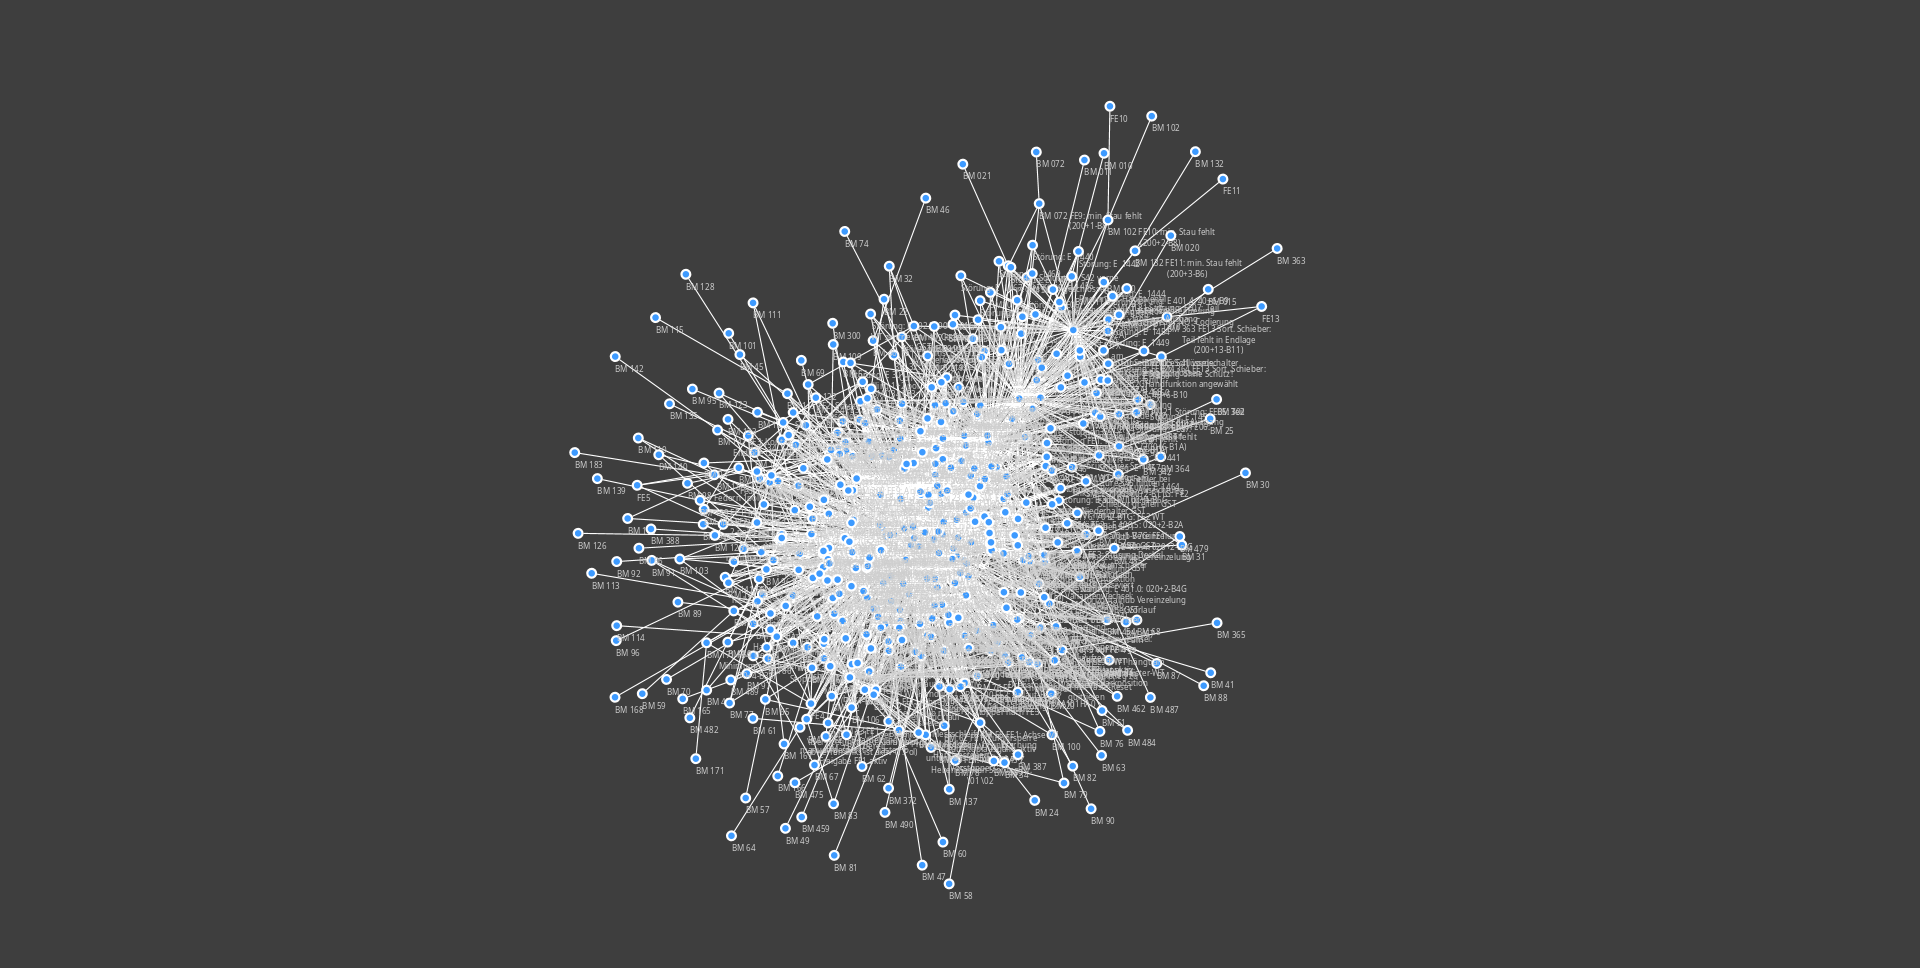
\includegraphics[width=\linewidth]{images/fullgraph}
    %\caption{Naive single graph encoding all available information}
    \label{fig:fullgraph}
\end{figure}
\end{frame}

\section{gSpan und SVM}
\begin{frame}{Graph-Aufbau}
\begin{itemize}
    \item Die Daten wurden unter Verwendung von Wissen um den Anlagen-Aufbau als \textit{constraints} in eine Graph-Form gebracht
    \item Jeder Graph enkodiert 5 Minuten an Informationen
    \item Auf der Menge der generierten Graphen wird dann der \textit{gSpan}-Algorithmus zur Pattern-Suche ausgeführt
\end{itemize}
\end{frame}

\begin{frame}{Graph-Isomorphismus}
\begin{itemize}
    \item Das Grundproblem beim Graph-Mining ist die Feststellung, ob zwei (Sub-)Graphen zueinander isomorph sind
    \item Def.: Seien $G$ und $H$ Graphen. Sei $f: V(G) \rightarrow V(H)$ eine Bijektion und $u, v \in V(G), (u,v) \in E(G)$. Dann gilt $G \simeq H$ g.d.w $(f(u), f(v)) \in E(H)$.
    \item Das Subgraph-Isomorphie-Problem ist NP-complete
\end{itemize}
\end{frame}

\begin{frame}{gSpan}
\begin{itemize}
    \item \textit{gSpan} ist ein pattern-growth Algorithmus von \textit{Yan und Han} aus 2002
    \item \textit{gSpan} weist jedem Graph ein kanonisches, auf DFS traversal basierendes Label zu (DFS-Codes)
    \item Zwei Graphen mit gleichem Label sind isomorph
    \item \textit{gSpan} findet sodann alle Subgraphen der Elemente einer Menge von Graphen, welche einen \textit{minimum support threshold} (\textit{min\_sup}) erreichen.
\end{itemize}
\end{frame}

\begin{frame}{Modifikation von gSpan}
\begin{itemize}
    \item Beim Implementieren von \textit{gSpan} in Python fiel auf, dass die DFS-Codes ähnlich wie Hashes funktionieren, aber die verwendete Datenstruktur Vergleichsoperationen nicht sehr effizient macht
    \item Leider kann gSpan nicht vollständig auf den reinen Vergleich von Hashes umgestellt werden, da über der Menge der DFS-Codes eine starke Totalordnung liegen muss
\end{itemize}
\end{frame}

\begin{frame}{Beispiel DFS-Code}
\begin{figure}
    \centering
    \begin{tikzpicture}[node distance = 2cm]
    \tikzset{VertexStyle/.style = {
            shape=circle,
            draw=black
    }}
    \node[VertexStyle, label={[label distance=-.2cm]45:\small $v_1$}] (1){X};
    \node[VertexStyle, right of= 1, label={[label distance=-.2cm]45:\small $v_2$}] (2){Y};	
    \node[VertexStyle, right of= 2, label={[label distance=-.2cm]45:\small $v_3$}] (3){Z};
    \node[VertexStyle, below of= 2, right of=2, label={[label distance=-.2cm]45:\small $v_4$}] (4){U};
    
    \path [-] (1) edge node[above] {a} (2);
    \path [-] (2) edge node[above] {b} (3);
    \path [-] (3) edge node[left] {c} (4);
    \path [-] (2) edge node[left] {d} (4);
    \end{tikzpicture}
    %\caption[Graph $G$ from chapter \ref{chapter:theoretical_basis} with labels]{Graph $G$ from chapter \ref{chapter:theoretical_basis} with labels}
    \label{fig:example_graph_dfs}
\end{figure}
\begin{table}[h]
    \centering
    %\caption{Minimum DFS code of graph $G$}
    \label{table:dummy_min_dfs_codes}
    \begin{tabular}{l|l}
        edge no. & DFS code          \\ \hline
        0        & $(0,2,U,d,Y)$     \\
        1        & $(1, 2, X, a, Y)$ \\
        2        & $(0, 3, U, c,Z)$  \\
        3        & $(2, 3, Y, b, Z)$
    \end{tabular}
\end{table}
\end{frame}

\begin{frame}{Pattern-growth Aspekt}
\begin{itemize}
    \item Beim Suchen nach neuen Patterns verwendet \textit{gSpan} die schon gefundenen Patterns
    \item Pattern-Kandidaten können neue Kanten nur am \textit{rightmost path} anfügen, was den Suchraum eingrenzt
\end{itemize}
\end{frame}

\begin{frame}{Support Vector Machine}
\begin{itemize}
    \item Zum Klassifizieren der Patterns zu den gefundenen Anomalien wurde eine SVM eingesetzt
    \item Eine SVM ist ein supervised learning Modell, das relativ effizient hochdimensionale Datenpunkte auf zwei Klassen verteilen kann
\end{itemize}
\end{frame}

\section{Ergebnisse}

\begin{frame}{Beispiel-Pattern}
\begin{figure}
    \centering
    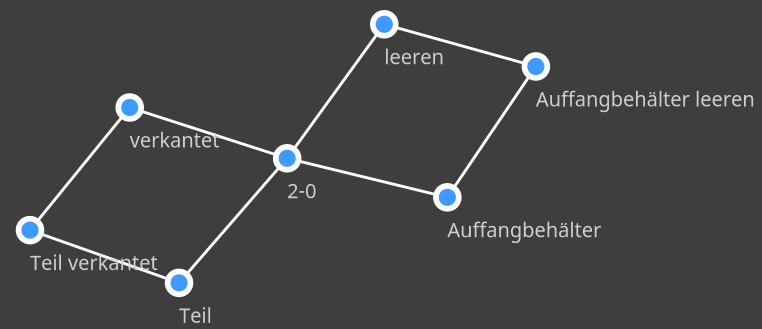
\includegraphics[width=1\linewidth]{images/dummy_pattern}
    %\caption{8-edge pattern from the synthetic data set, min\_sup = .4}
    \label{fig:dumm_pattern}
\end{figure}
\end{frame}

\begin{frame}{Synthetischer OEE-Verlauf}

\begin{figure}
    \centering
    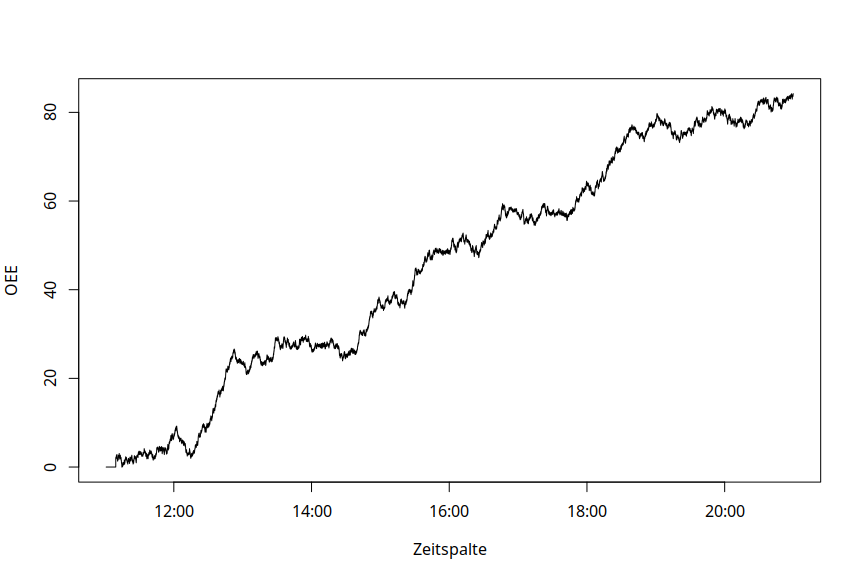
\includegraphics[width=1\linewidth]{images/dummy_random_walk}
    %\caption{Synthetic OEE values}
    \label{fig:dummyrandomwalk}
\end{figure}
\end{frame}

\begin{frame}{Laufzeiten synthetische Daten}
\begin{table}[]
    \centering
    %\caption{Run times and patterns found (synthetic data set)}
    \label{table:runtimes_syn}
    \begin{tabular}{l|l|l}
        data set                                      & \textit{t} & patterns \\ \hline
        import errors and graph generation            & 1s         &          \\
        import and anomalies detection on OEE scores  & 8s         &          \\ \hline
        \textit{gSpan} (min\_sup = .7)                & 2s         & 40       \\
        \textit{gSpan} (min\_sup = .6)                & 8s         & 106      \\
        \textit{gSpan} (min\_sup = .5)                & 19s        & 241      \\
        \textit{gSpan} (min\_sup = .4)                & 74s        & 1056     \\ \hline
        SVM training and validation   (min\_sup = .7) & 4s         &          \\
        SVM training and validation   (min\_sup = .6) & 8s         &          \\
        SVM training and validation   (min\_sup = .5) & 35s        &          \\
        SVM training and validation   (min\_sup = .4) & 13m 14s    &
    \end{tabular}
\end{table}
The validation data set consisted of 49 time windows, 33 of which were deemed as a noticeable drop by the OEE evaluation algorithm. Of these 33, the SVM correctly identified 28 as drops, for a sensitivity score of 84.85\%. Of the remaining 19 non-drops, 5 were falsely identified as positives, for a specificity score of 73.68\%.
\end{frame}

\begin{frame}{Laufzeiten reale Anlagendaten}
\begin{table}
    \centering
    %\caption{Run times and patterns found (facility data set)}
    \label{table:runtimes_real} 
    \begin{tabular}{l|l|l}
        data set                                      & \textit{t}          & patterns \\ \hline
        import errors and graph generation            & 50s                 &          \\
        import and anomalies detection on OEE         & 2m 27s              &          \\ \hline
        \textit{gSpan} (min\_sup = .9)                & 2m 20s              & 12       \\
        \textit{gSpan} (min\_sup = .7)                & 6h 27m 12s          & 846      \\
        \textit{gSpan} (min\_sup = .5)                & \textit{OOM killed} & --       \\ \hline
        SVM training and validation   (min\_sup = .7) & 27s                 &
    \end{tabular}
\end{table}
The validation data set consisted of 486 time windows, 64 of which were deemed as a noticeable drop by the OEE evaluation algorithm. Of these 64, the SVM trained on patterns with a min\_sup of .7 correctly identified 60 as drops, for a sensitivity score of 93.75\%. Of the remaining 422 non-drops, 18 were identified as false positives, for a specificity score of 95.73\%.
\end{frame}

\end{document}
